% !TEX root = Thesis.tex

\chapter{Visual Synthesis}
\minitoc

\begin{figure}[ht]
 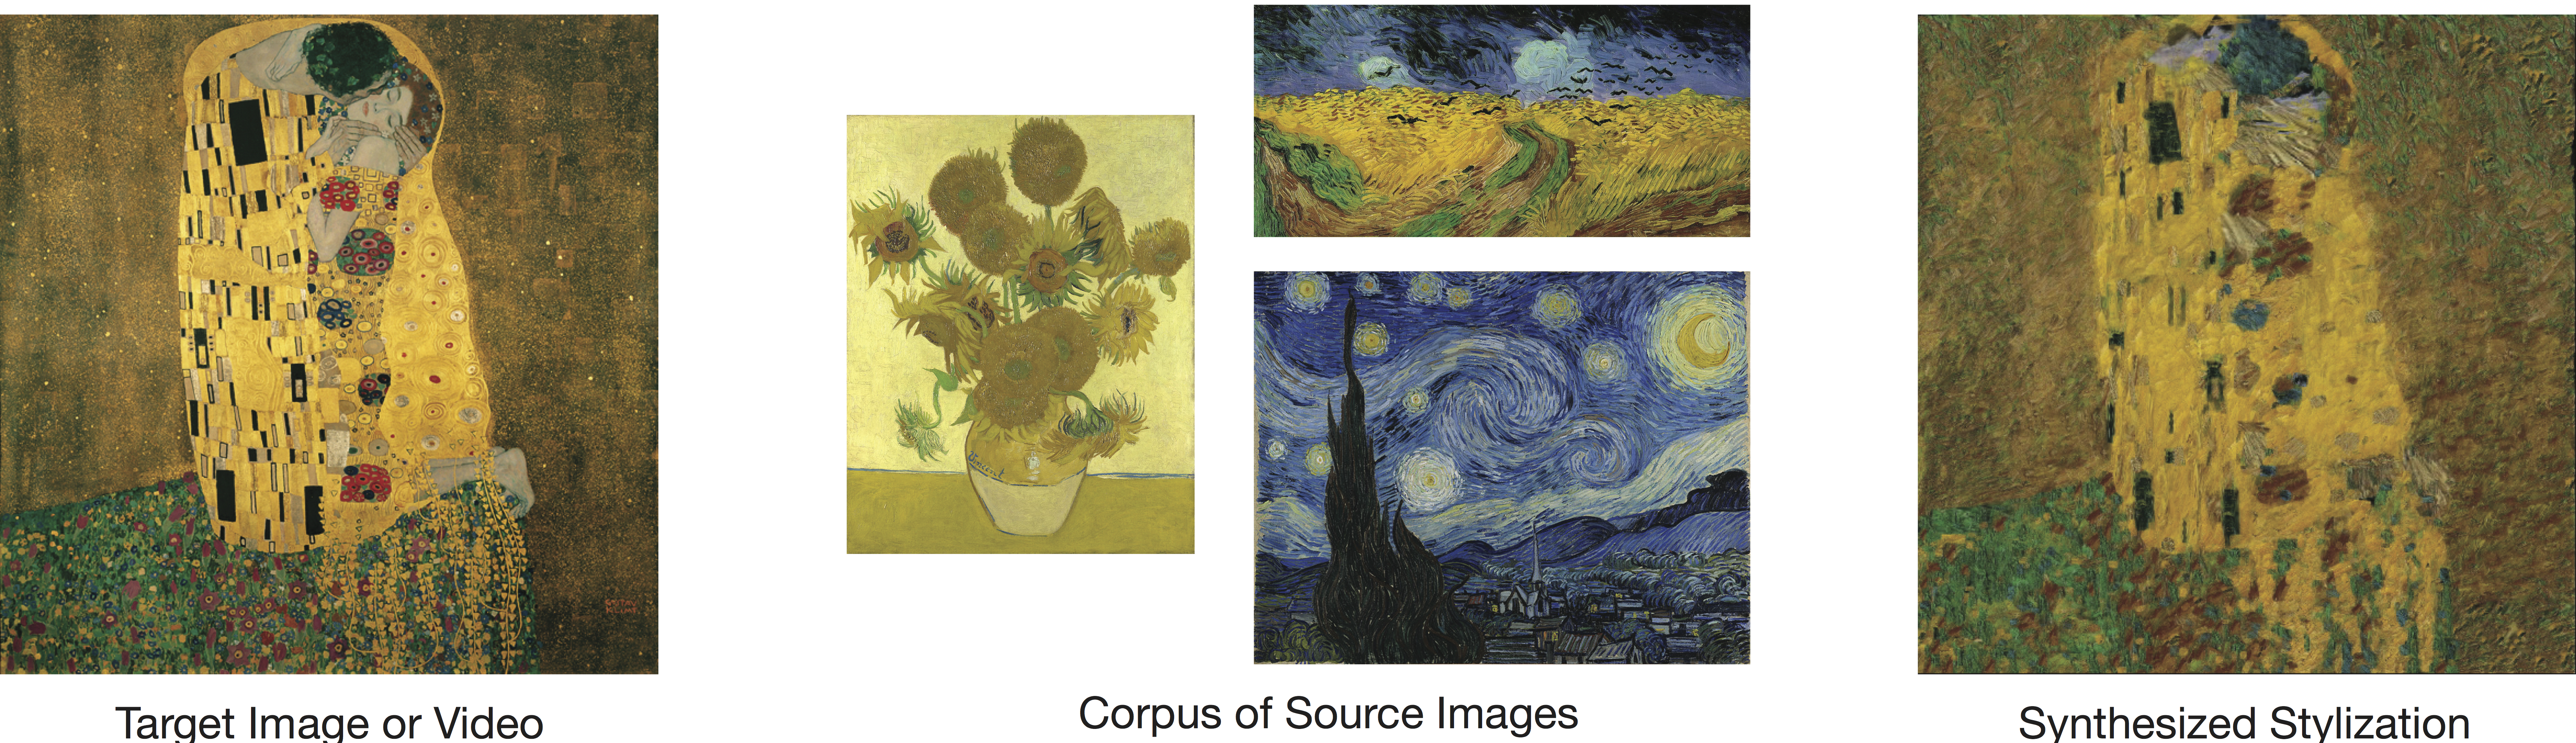
\includegraphics[width=\textwidth]{images/klimt-van-gogh-wide.png}
 \caption{Klimt's ``The Kiss'' is synthesized using 3 images of Van Gogh paintings to produce the result on the right.  Best viewed in color at 400\%.  Images representing faithful reproductions of Gustav Klimt and Van Gogh sourced from \href{http://commons.wikimedia.org}{Wikimedia Commons} are public domain.}
 %https://en.wikipedia.org/wiki/File:Gustav_Klimt_016.jpg
 %https://en.wikipedia.org/wiki/File:Vincent_van_Gogh_(1853-1890)_-_Wheat_Field_with_Crows_(1890).jpg
 %https://en.wikipedia.org/wiki/File:Van_Gogh_-_Starry_Night_-_Google_Art_Project.jpg
 %http://www.nationalgallery.org.uk/paintings/learn-about-art/paintings-in-depth/sunflowers-symbols-of-happiness
 \label{fig:teaser}
\end{figure}

\begin{abstract}
We investigate an approach to the artistic stylization of photographic images and videos that uses an understanding of the role of abstract representations in art and perception.  We first learn a database of representations from a corpus of images or image sequences.  Using this database, our approach synthesizes a target image or video by matching geometric representations in the target to the closest matches in the database based on their shape and color similarity.  We show how changing a few parameters of the synthesis process can result in stylizations that represent aesthetics associated with Impressionist, Cubist, and Abstract Expressionist paintings.  As the stylization process is fast enough to work in real-time, our approach can also be used to learn and synthesize the same camera image, even aggregating the database with each new video frame in real-time, a process we call "Memory Mosaicing".  Finally, we report the user feedback of 21 participants using an augmented reality version of "Memory Mosaicing" in an installation called �Augmented Reality Hallucinations�, where the target scene and database came from a camera mounted on augmented reality goggles.  This information was collected during an exhibition of 15,000 participants at the Digital Design Weekend at the Victoria and Albert Museum (co-located during the London Design Festival).
\end{abstract}

\section{Introduction}  
Despite its apparent precision, our perception of reality is not representative of the way that we see.  For instance, the light coming to our eyes is distorted, upside-down, and constantly disrupted with each movement of the eye.  How can this noisy process ever constitute our experience of the visual world?  Numerous theories have argued that in order to perceive the world as a continuous and richly detailed one, our vision system must use abstracted representations of the world \cite{Marr1982}.  It is argued that these representations are created by grouping together coherent visual features that resemble abstract forms - such as geometrical primitives. Grouping such primitives together eventually leads to the formation of semantic representations such as objects. Importantly, the representations used in vision are not necessarily what we perceive, but are what we use in order to help us perceive. As a result, these representations are likely to remove details that are unimportant to a person's ongoing task while making other details more explicit.

Artists are well aware of the role of representation in perception.  By leaving out particular details from a visual scene and accentuating others, they are able to direct a viewer's attention within a visual medium, influencing their perception \cite{Haeberli1990,Zimmer2003}.  Picasso once famously said, "I paint forms as I think them, not as I see them" \cite{Hughes1991}.  As one of the pioneers of Cubism, Picasso wanted to represent the fact that our perception of an object is based on all possible views of it.  He did so by compressing all views of an object into a synthesized one built using abstracted shape primitives.  Other movements in art can also be characterized as utilizing representations formed through geometrical primitives.  In Impressionist painting, these forms are often described by a dense number of short and visible brush strokes.  In Abstract Expressionist painting, the primitives are again dense, though tended to be of much larger strokes in an attempt to abstract away as much detail of a real scene as possible.

In this paper, we investigate an approach to the artistic stylization of photographic images and videos through the use abstracted shape representations.  The representations that are built by this method can be varied in size and density using a process that allows the user to manipulate parameters in real-time.  Our system first learns a database of representations from a corpus of images.  It then synthesizes a target image or video by matching geometric representations in the target to the closest matches in the database.  We show how changing the parameters of the synthesis process results in stylizations that represent aesthetics associated with Impressionist, Cubist, and Abstract Expressionist paintings.  As the stylization process is fast enough to work in real-time, this approach can also be used to learn and synthesize the same camera image, even aggregating the database with each new video frame in real-time, a process we call "Memory Mosaicing".  Finally, we report the feedback of 21 participants using an augmented reality version of "Memory Mosaicing" in an installation called �Augmented Reality Hallucinations�, where the target scene and database came from a camera mounted on augmented reality goggles.
\section{Related Work}  
Artistic stylization has seen significant advances over the last 14 years.  Kyprianidis recently surveyed the field in \cite{Kyprianidis2012}.  The field began as filtering and clustering algorithms were applied to images, accentuating regions within an existing image to produce aesthetics associated with different styles (e.g., for Pointillism \cite{Yang2006,Seo2010}; for cartoonization \cite{Wang2004}; for oil and watercolor \cite{Meier1996,Hertzmann2000,Bousseau2007,Gooch2002}; for Impressionism \cite{Litwinowicz1997,Hertzmann1998}).  More recent approaches focused on using user-guided segmentation, where the user manually labels key frames with strokes defining how the frame is stylized (e.g. \cite{O'Donovan2012}) or uses eye-movements in deciding which aspects of a photo are most salient \cite{DeCarlo2002}.

Hertzmann's seminal work in Image Analogies \cite{Hertzmann2001} presented a branch from the aforementioned approaches by allowing control of the stylization process through choosing a pair of example images.  By finding the patterns associated with an existing stylization of an image A to another image A', a user could then stylize a target image B by analogy into B' (later extended to include analogies between curved strokes \cite{Hertzmann2002}).  In the same year, \cite{Efros2001,Liang2001a} also developed methods in texture transfer and patch-based sampling, where existing image material was used to synthesize textures of arbitrary sizes.  These methods were later extended in \cite{Wang2004a}, where a user specified small blocks in an example painting that represented the style to recreate.  These blocks were then synthesized along computed paint strokes in the target image using an efficient hierarchical texture synthesis method.  Though Wang's approach and even more recent methods (e.g., \cite{Guo2006}) produces impressive results, it also relies on user interaction to select the representative patches expressing an artistic style.  Further, the aforementioned work in texture transfer as well as more recent approaches (e.g., \cite{Lee2010}) all rely on a single source image in order to transfer the style of the texture, meaning the range of stylizations possible are constrained to the information contained in a single image.  In this paper, we develop an approach that does not require the user to manually label any regions and that is not confined to a single example image while still affording a range of possible styles.  

Our approach, corpus-based visual synthesis (CBVS), synthesizes a target image/video using existing pre-defined visual content.  As a result, it is also borrows methods from dictionary-based approaches (\cite{Zeng2009,Healey2004}), though our approach does not focus on developing strokes from expert training as we automatically segment a corpus of user chosen images.  It also shares methodology with collage/mosaic-based work (e.g. \cite{Kim2002,Orchard2008,Huang2011a,Miller2012}), allowing a user to work with a period of an artist's work or entire videos, for example.  Though these approaches are targeted for collage/mosaic-based purposes rather than artistic stylization, \cite{Huang2011a} describes an approach that is also motivated by an artist making use of collage.  Their approach produces what they call ``Arcimboldo-like'' collages in the style of 18th century painter Giuseppe Arcimboldo, relying on user strokes to segment the images used.  In contrast, CBVS is aimed towards producing a range of possible artistic stylizations through changing a few simple parameters.  Further, as segmentation happens without requiring user-selected patches or strokes, CBVS is also suitable for producing stylization of videos, unlike the very impressive though slow approach (15 minutes for a 300 x 400 pixel image) reported in \cite{Chang2010}.
\section{Corpus-based Visual Synthesis Framework}  
CBVS begins by first aggregating all frames from a user chosen corpora of images, $\mathbf{C} = \{C_1, C_2, ..., C_N\}$, containing $N$ total candidate images.  We aim to use the content solely from this corpus to artistically stylize a target image or video, $\mathbf{T} = \{T_1, T_2, ..., T_M\}$, containing $M$ total frames.  We develop a rendering procedure for image and video-based targets where parameters of the synthesis can be changed interactively.  To begin, we describe detection, tracking, description, matching, and synthesis of the abstracted shape representations.  We then describe parameters influencing each of these steps before showing our results in Section \ref{sec:results}.
\subsection{Detection}\vspace{-0.4em}
For both the candidate and target frames, we aim to detect abstracted shape primitives described by coherent image regions.  For this purpose, we make use of maximally stable color regions (MSCR) \cite{Forssen2007}.  The algorithm described in \cite{Forssen2007} successively clusters neighboring pixels with similar colors described by multiple thresholds of a distance measure which takes into account the inherent camera noise and the probability distribution of each RGB color channel.  Regions are denoted as maximally stable if they do not grow larger than a minimum margin for certain number of time-steps.  Previous techniques employing posterization, filtering, or watershed have had to apply their algorithm at multiple scales in order to discover regions that are superimposed or overlapped, increasing their computational complexity.  MSCR has the benefit over these previous techniques as it provides an implicit ordering of superimposed regions discovered through successive time-steps of the clustering algorithm.  Further, it allows us to prune regions by restricting their area to a range of minimum and maximum sizes.  In Section \ref{sec:parameters}, we discuss these parameters in greater detail in relation to the styles they can produce. 
We use MSCR to detect the set of all regions in each candidate and target frame, denoted as $\mathbf{R_C} = \{R_1, R_2, ..., R_{N_C}\}$ and $\mathbf{R_T} = \{R_1, R_2, ..., R_{N_T}\}$ where $N_C$ is the number of regions detected in all candidate frames and $N_T$ is the number of target regions.  
\subsection{Tracking}\vspace{-0.4em}
It is often desirable to produce temporally coherent stylizations, meaning if a region within a target video frame has not moved, it is not re-stylized.  This is especially the case in noisy or compressed videos, where artifacts may appear that should not be stylized.  One approach would be to track regions using a GPU-based Optical Flow measure.  This would likely produce reasonable temporal coherence without sparing real-time interaction.  However, we simply follow \cite{Hertzmann2000} in using the flicker for detecting the change in the original target video, as this approach is fast and easy to compute.  Let the flicker for a pixel at location $(i,j)$ be described by:
\begin{equation}
f(i,j) = I_t(i,j) - I_{t-1}(i,j)
\end{equation} 
where $I$ is the image luminance at time $t$.  Then, if the flicker at the region's centroid, $f(C_{R_i})$, between the current and previous frame is greater than a threshold, $threshold$, we remove the region from the set of detected regions to synthesize:
\begin{equation}
R_T = \{ R_i \suchthat f(C_{R_i}) > threshold, \forall i = 1...N_T \}
\end{equation}
\subsection{Description}\vspace{-0.4em}
We form a descriptor comprised of shape and color values.  The shape descriptor for each region, $d_{R_i}$, is composed of the normalized central moments up to order 2.  The average color of the region is converted from RGB to the 3-channel CIELAB color space, $L, a^{*}, b^{*}$.  These form the final descriptor: 
\begin{equation}
d_{R_i} = \Big(\mu_{00}, \eta_{11}, \eta_{20}, \eta_{02}, L, a^{*}, b^{*}\Big)
\end{equation}
where $\mu_{ij}$ is the central image moment of order $i$ and $j$, i.e. $\mu_{00}$ is simply the area, and $\eta_{ij}$ is the normalized central image moment computed as: 
\begin{equation}
\eta_{ij} = \frac{\mu_{ij}}{\mu_{00}^{\left(1 + \frac{i+j}{2}\right)}}
\end{equation}
Centralizing the moments allows us to compare regions with translation-invariance, while normalizing the first and second order moment allows us to compare regions with scale-invariance.  We include the area as the first term as this ensures regions are not distorted too much when matching.  Further, employing CIELAB allows us to define the region in a color space where we can then use perceptual metrics for matching.  We describe this metric in greater detail in the next section.
\subsection{Matching}\vspace{-0.4em}
We match each region in the target to its nearest neighbors in the database using a metric combining distances from each region's shape and color, $d_s(R_t, R_c)$ and $d_c(R_t, R_c)$, respectively:  
\begin{equation}
d(R_t, R_c) = d_s(R_t, R_c) + d_c(R_t, R_c)
\end{equation}
\label{eq:distance}
The shape distance is simply computed as the absolute difference between the first and second order normalized central image moments of each region (i.e. the first four components of the descriptor).  For the color distance, we make use of the official CIE color-difference equation, CIEDE2000, which provides reliable color discrimination with interactive terms for lightness, chromaticity, and hue weighting \cite{Luo2001}.   This difference formula has been shown to be more perceptually accurate at determining the difference between colors than previous methods employing linear difference using RGB or LUV color values, as it is based on empirical evidence of perceived color difference.  For our tests, we use the default parameters described in \cite{Luo2001} for the weighting terms.
\subsection{Synthesis}\vspace{-0.4em}
To ensure regions are drawn from their background to the foreground, we synthesize each target region in order from the largest to smallest area sizes.  In contrast to methods that place brush strokes based on the stroke direction at each pixel on the medial axis (e.g.,\cite{Wang2004a}), we find the affine geometric transform describing the transformation from $R_{C_i}$ to $R_{T_i}$.  This can be described by a translation, rotation, and scaling.  The translation component is simply the difference in each region's centroid.  The rotation can be found using the central image moments: 
\begin{equation}
\Theta = \frac{1}{2} * \arctan  \dfrac{ 2 * \frac{\mu_{11}}{\mu_{00}} } { \frac{\mu_{20}}{\mu_{00}} - \frac{\mu_{02}}{\mu_{00}} }
\end{equation}
Finally, scaling is simply the ratio of the target to candidate region's bounding box.  This process has the benefit of being very fast using graphics hardware as it can be computed by a single matrix multiplication.  Each region is then layered above the previous one before creating a synthesized image.  In image-based stylization, multiple syntheses created with changing parameters can be blended together to create more detailed and expressive styles which may require many ``layers'' of ``paint''.  We discuss these parameters in greater detail in the next section.
\section{Parameters}  
Parameters influencing the region detection algorithm are set independently for the corpus and the target, as their function differs.
\subsection{Corpus Parameters}\vspace{-0.4em}
\label{sec:parameters}
For the corpus, we define the \textit{timesteps}, \textit{minimum region area}, and \textit{maximum region area} of the detected regions.  We use a set of parameters that learns the widest range of possible regions covering both small and large regions.  In some cases, as in more abstract styles, it may be desirable to learn a very small number of regions, limiting the range of expressiveness to a few possible primitives.  As the timesteps parameter influences the number of evolutions allowed in the MSCR algorithm, the higher this number, the more regions will be discovered.  Similarly, lowering the minimum region size and increasing the maximum region size reduces the number of region that are pruned.  In our tests, we found a single set of parameters to be sufficient for defining a varied corpus: 100 for the timesteps, 35 pixels for the minimum region area, and 50\% of the image's size for maximum region area.

When learning a corpus from many images, we restrict learning regions that are within a distance threshold (using Equation \ref{eq:distance}) of all regions in the existing database.  For our examples, we set this parameter to 50.  This value is low enough to include many regions, though high enough to avoid detecting duplicate regions.  A higher number for this parameter will lead to very discriminative regions.  In our tests, when setting this number higher, we found that our corpus had less variety of regions to synthesize from, leading to stronger shape or color mismatches.  
\subsection{Target Parameters}\vspace{-0.4em}
\begin{figure}[ht]
  \centering
  \includegraphics[width=3.1in]{images/spatial-blending-3.png}
  
  \caption{Using the target image and database shown in Figure-\ref{fig:teaser}, we show an example stylization with (first image) and without (second image) spatial blending.  We also draw the region's orientation depicted by red/green axes in order to better show the regions (best viewed in the color manuscript at 200\%).}
  \label{fig:spatial-blending}
\end{figure}
\begin{figure}[ht]
  \centering
  \includegraphics[width=3.1in]{images/increasing-timesteps-2.png}
  
  \caption{Using the target image and database shown in Figure-\ref{fig:teaser}, the timesteps are increased over time.  This allows the user to detect more regions and develop a denser and higher contrast stylization.}
  \label{fig:timesteps}
\end{figure}
\begin{figure}[ht]
  \centering
  \includegraphics[width=3.1in]{images/decreasing-minimum-size-2.png}
  
  \caption{Using the target image and database shown in Figure-\ref{fig:teaser}, the minimum region size is decreased over time, allowing the user to detect smaller regions and produce finer detailed stylizations.}
  \label{fig:minimum-size}
\end{figure}
\begin{figure}[ht]
  \centering
  \includegraphics[width=3.1in]{images/blending-radius-2.png}
  
  \caption{Using the target image and database shown in Figure-\ref{fig:teaser}, the blending radius is increased over time.  This parameter influences the overall size of the drawn regions.  Setting this number smaller can help to produce finer details on top of existing layers, often associated with both Impressionist and Abstract Expressionist styles.}
  \label{fig:blending-radius}
\end{figure}
\begin{figure}[ht]
  \centering
  \includegraphics[width=3.1in]{images/temporal-blending.png}
  
  \caption{Using the target image and database shown in Figure-\ref{fig:teaser}, we increase the temporal blending factor.  This influences the opacity of every region drawn. }
  \label{fig:temporal-blending}
\end{figure}
\begin{figure}[ht]
  \centering
  \includegraphics[width=3.1in]{images/temporal-blending-changing-params.png}
  
  \caption{Using the target image and database shown in Figure-\ref{fig:teaser}, we use temporal blending as well as decreasing minimum region size and increased timesteps to begin to produce the final synthesis.}
  \label{fig:temporal-blending-changing-parameters}
\end{figure}
For the target, we allow the user to interactively define a few parameters affecting the output stylization.  
\begin{itemize}
\item \textit{Spatial blending}: Allows the user to use feathered elliptical regions instead of rectangular ones (see Figure-\ref{fig:spatial-blending}).  When stylizing finer details of an image, this parameter is very useful for removing hard edges produced by rectangular regions.  
\item \textit{Timesteps}: Increasing this produces more regions, making the image denser (see Figure-\ref{fig:timesteps}).  As well, this will also produce more regions that coincide with each other.  As a result, when synthesizing with a high number for the timesteps, the result resembles an overpainting effect.  For styles that require many ``layers'' of ``paint'', we use a higher number for the timesteps.  When used in combination with blending, increasing this can also increase the contrast.
\item \textit{Minimum region size}: This parameter determines the minimum allowed region size for synthesis.  Setting this number very low (e.g. below 100 pixels) produces styles more similar to Impressionism, as many small regions are detected (see Figure-\ref{fig:minimum-size}).  
\item \textit{Maximum region size}: Similar to the minimum region size parameter, this parameter determines the largest allowed region size. Generally setting this number as high as possible will be sufficient.  However, it may be desirable to interactively change this parameter over time, allowing for large regions to be drawn at first, then only allowing smaller ones. 
\item \textit{Temporal blending}: Uses alpha blending to composite regions over time (see Figure-\ref{fig:temporal-blending}).  Together with an increased number of timesteps, this parameter can be used to change the contrast of the overall image (as shown in Figure-\ref{fig:temporal-blending-changing-parameters}).  
\item \textit{Motion tracking}: Allows regions to be drawn only if their detected motion is higher than a fixed threshold.  For our experiments, we set this number to 5.  
\item \textit{Blending radius}: Influences the feathering radius of the detected region (see Figure-\ref{fig:blending-radius}).  Normally, each detected region is matched to one in the database and then through an affine transformation placed where the detected region was using the same scale and rotation.  However, it may be desirable to change the scale of this region using the blending radius to produce different effects.  When scaling this region down, a user confines drawing to only small regions being painted, often produces styles associated with Abstract Expressionism.
\end{itemize}
For image-based targets, the aforementioned parameters effect the frame-to-frame compositing, meaning the same image is rendered over itself.  For video-based targets, however, only a single iteration is used for each frame, as much of the information required for building styles requiring more detailed composites can be extracted over the first 1 or 2 frames.  We demonstrate how these parameters can influence a wide range of stylizations in the next section.
\section{Results}  
\label{sec:results}
We use the presented framework to produce artistic stylizations of photo-realistic images and videos.  In this section, we show our results in image-based stylization using a landscape, abstract, and painterly scene. We then show how the same framework can be used with video targets, including an abstract and portrait video.  As well, we show a particular case where the source material is aggregated from a live-stream of the target, i.e. the source and target are the same, a process we call ``Memory Mosaicing''.  Finally, we present an augmented reality version of ''Memory Mosaicing'' including feedback collected from 21 participants of an installation at the Victoria and Albert Museum in London. 
\subsection{Image: Landscape}\vspace{-0.4em}
\begin{figure*}[ht]
  \centering
  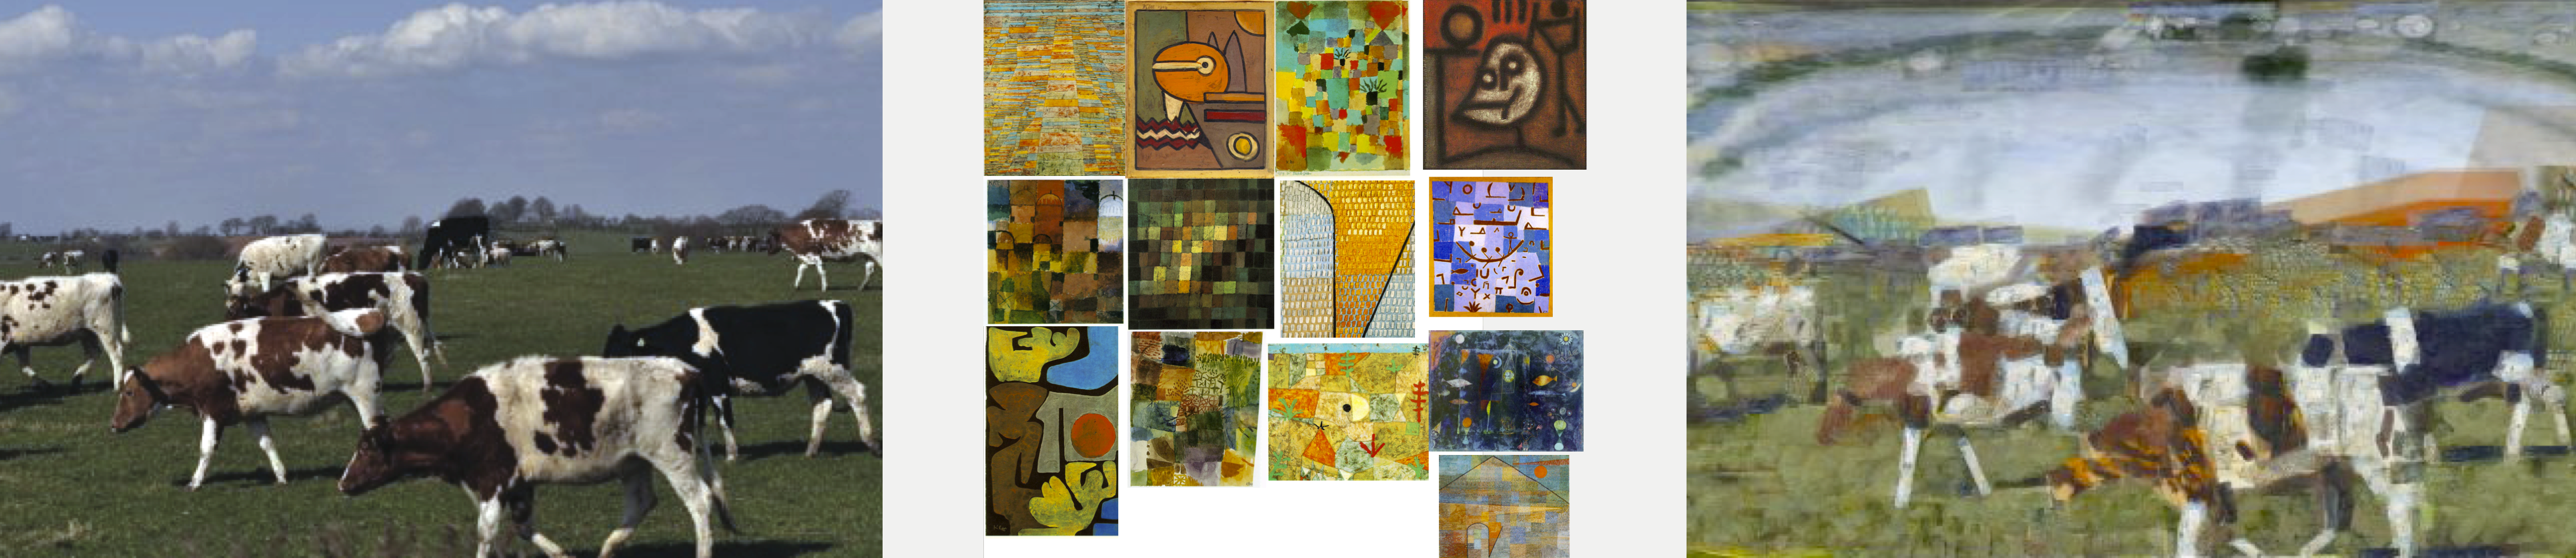
\includegraphics[width=\textwidth]{images/cows-klee.png}
  \caption{A landscape picture of cows grazing is synthesized using 13 images of Expressionism painter Paul Klee to produce the image on the right.  Images representing faithful reproductions of Paul Klee sourced from \href{http://www.artchive.com/}{Mark Harden's Artchive} are public domain. Photo of cows taken by the author.}
  %www.sai.msu.su/wm/paint/auth/klee/
  %This work is in the public domain in the United States because it was first published outside the United States (and not published in the U.S. within 30 days) and it was first published before 1978 without complying with U.S. copyright formalities or after 1978 without copyright notice and it was in the public domain in its home country on the URAA date (January 1, 1996 for most countries).
  %This work is in the public domain in the European Union and non-EU countries with a copyright term of life of the author plus 70 years or less.
  \label{fig:cows-klee}
\end{figure*}
In Figure-\ref{fig:cows-klee}, we synthesize a landscape photo of cows grazing using Expressionist painter Paul Klee.  We turn off spatial blending and use a small value for the minimum region size.  We also allow the maximum region size to be very large.  This results in a relatively smaller region being matched to the sky and stretched to fill the top-half of the image.  The synthesized region happens to look like a rainbow, though the original region itself was very abstract (see the first image in the second row of the Klee corpus).  
\subsection{Image: Abstract}\vspace{-0.4em}
\begin{figure*}[ht]
  \centering
  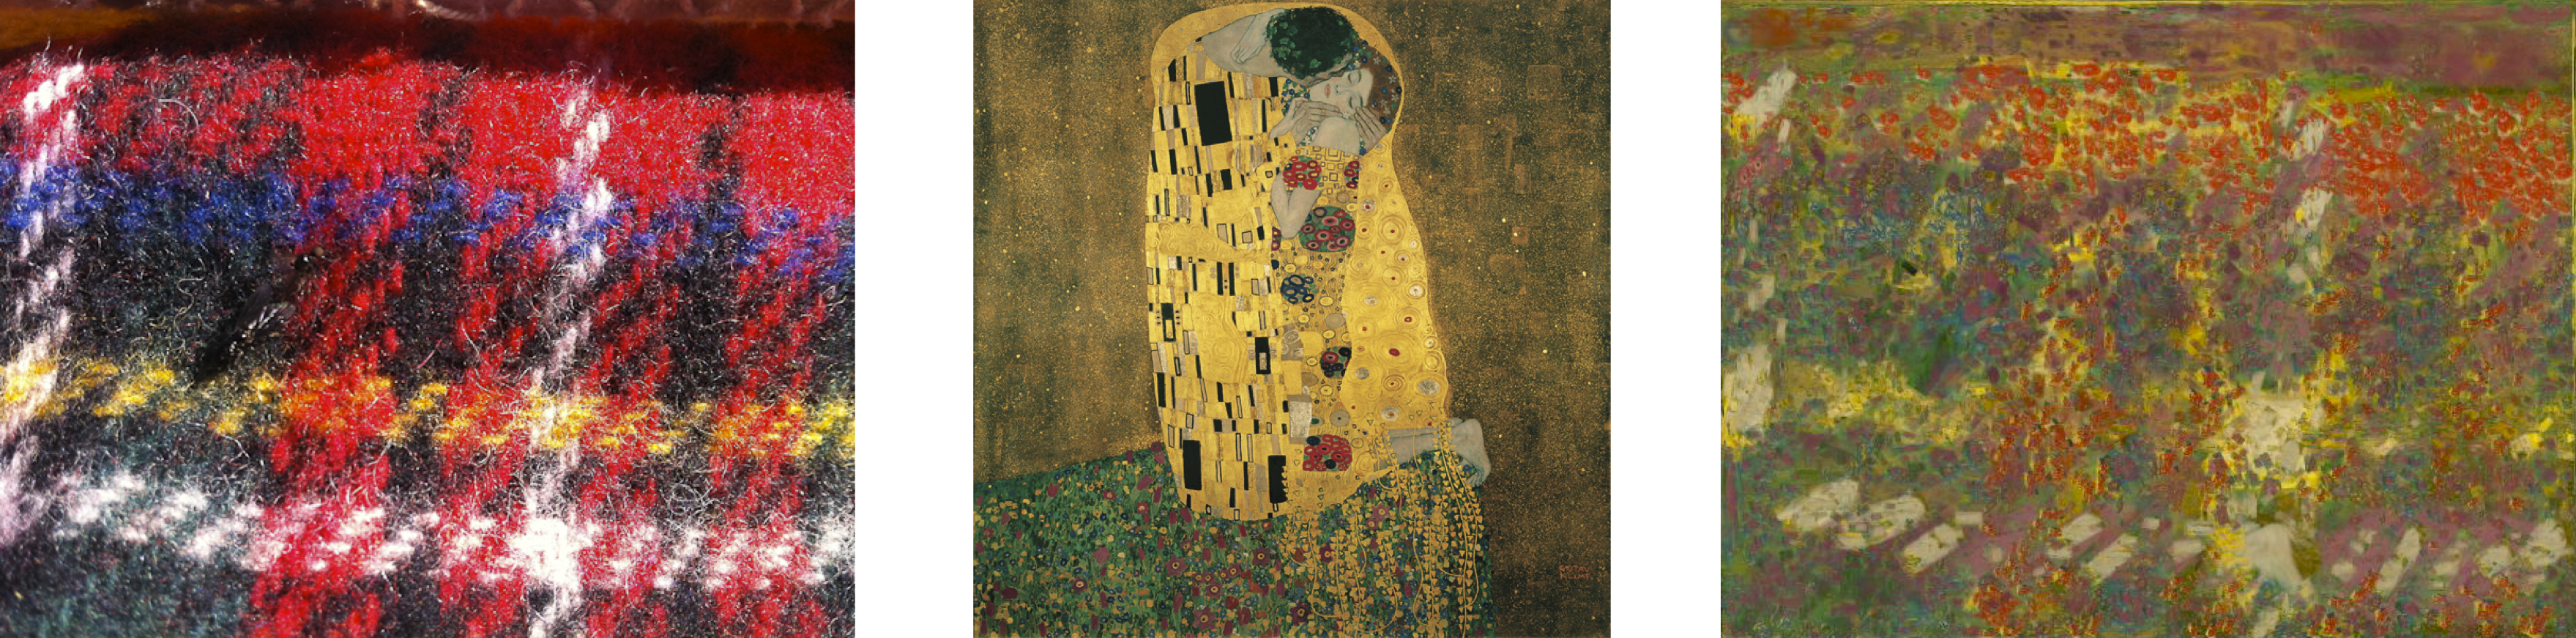
\includegraphics[width=\textwidth]{images/blanket-klimt.png}
  \caption{A close-up picture of a blanket is synthesized using Klimt's The Kiss to produce the image on the right. Best viewed in the color manuscript at 200\%. Images representing faithful reproductions of Gustav Klimt sourced from \href{http://commons.wikimedia.org}{Wikimedia Commons} are public domain.  Photorealistic scene of blanket taken by the author.}
  %https://en.wikipedia.org/wiki/File:Gustav_Klimt_016.jpg
  \label{fig:blanket-klimt}
\end{figure*}
In Figure-\ref{fig:blanket-klimt}, we synthesize a close-up picture of a blanket using Klimt's The Kiss.  The target this time is very abstract and we will not need to synthesize parameters that force an abstract quality rendering such as large region sizes.  As such, we allow the minimum region size to be very small producing more details, though retaining a style associated with Abstract Expressionism.
\subsection{Image: Painterly}\vspace{-0.4em}
\begin{figure*}[ht]
  \centering
  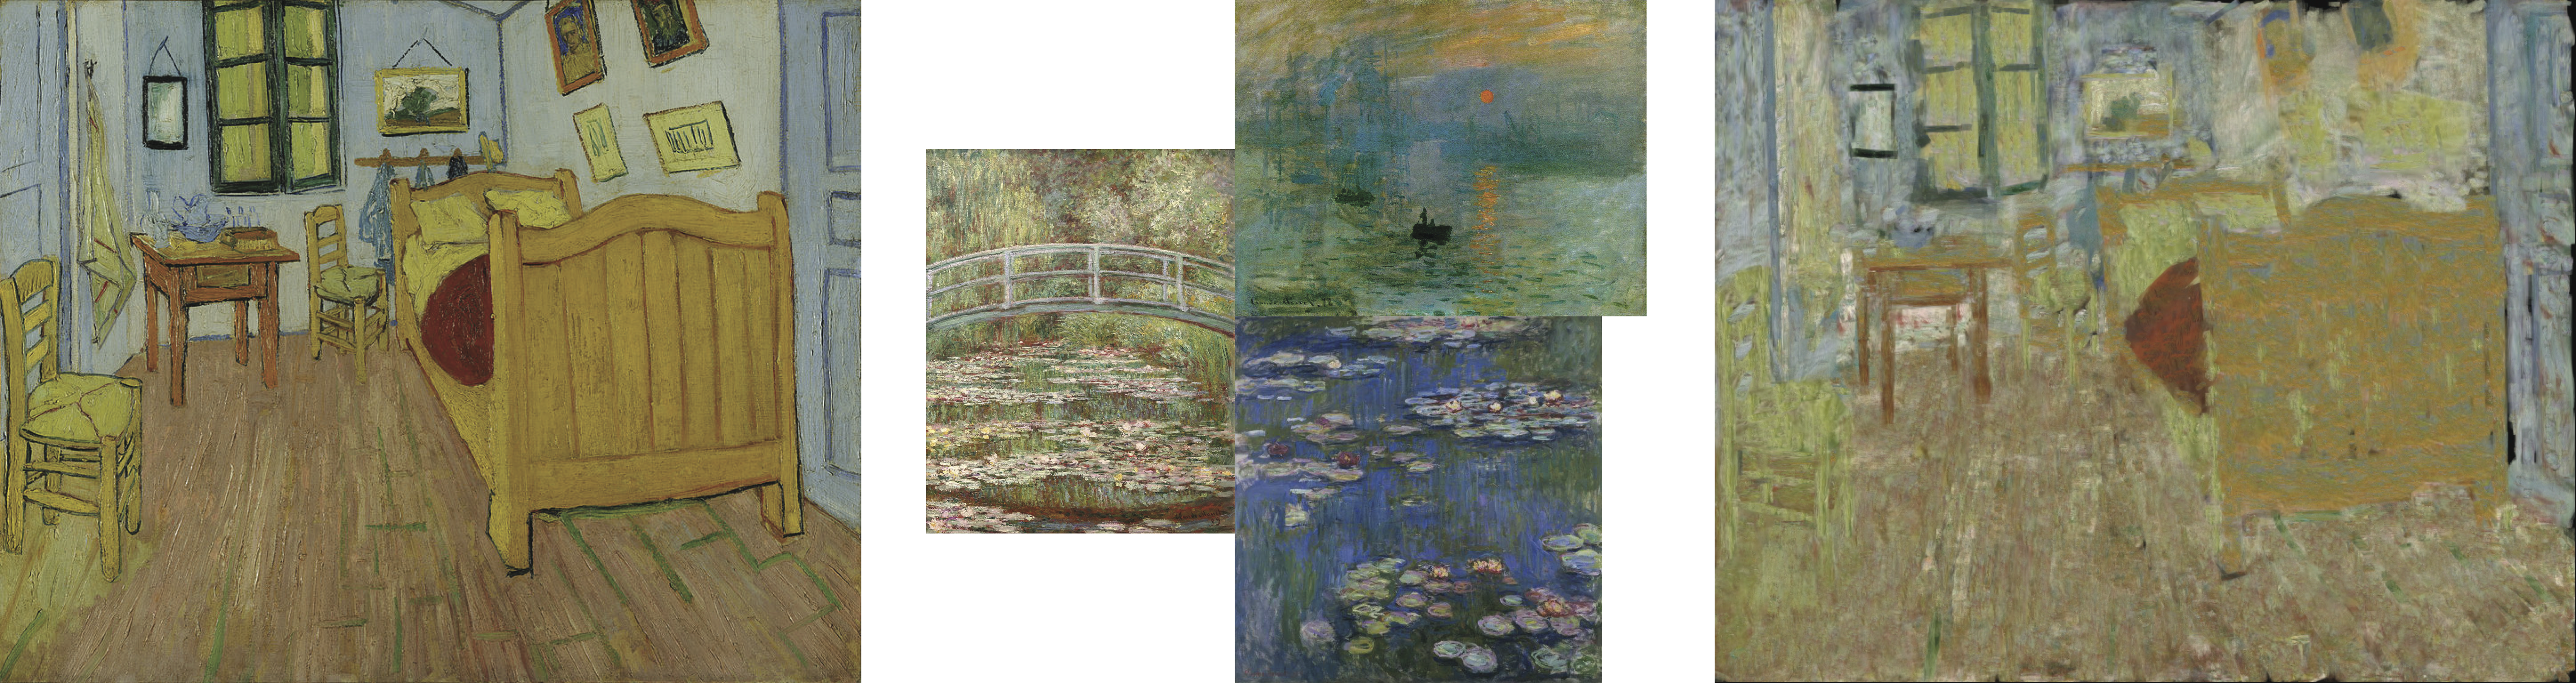
\includegraphics[width=\textwidth]{images/van-gogh-monet.png}
  \caption{Van Gogh's ``The Bedroom'' is synthesized using 3 images of Monet paintings to produce the image on the right. Images representing faithful reproductions of Van Gogh and Claude Monet sourced from \href{http://commons.wikimedia.org}{Wikimedia Commons} are public domain.}
  %https://commons.wikimedia.org/wiki/File:La_Chambre_%C3%A0_Arles,_by_Vincent_van_Gogh,_from_C2RMF.jpg
  %https://en.wikipedia.org/wiki/File:Claude_Monet,_Impression,_soleil_levant,_1872.jpg
  %https://en.wikipedia.org/wiki/File:Bridge_Over_a_Pond_of_Water_Lilies,_Claude_Monet_1899.jpg
  %https://en.wikipedia.org/wiki/File:Monet_Water_Lilies_1916.jpg
  \label{fig:van-gogh-monet}
\end{figure*}
We demonstrate how CBVS can stylize existing painterly images into other styles.  In the teaser graphic in Figure-\ref{fig:teaser}, we use three paintings by Van Gogh to stylize Klimt's The Kiss.  Here, we set the minimum region size to be small, allowing finer details and smaller brush strokes, and allow the timesteps to be high as we want to bring out as much contrast as possible.  

In Figure-\ref{fig:van-gogh-monet}, we try synthesizing Van Gogh's The Bedroom using 3 images of Monet's Water Lilies series.  Here, we ensure we detect many small regions by increasing the timesteps and setting the minimum region size to be very small.  Further, we turn on spatial blending as we decrease the minimum region size, as we want to avoid rendering any strong edges, retaining an Impressionist quality.
\subsection{Video: Portrait}
\begin{figure}[ht]
  \centering
  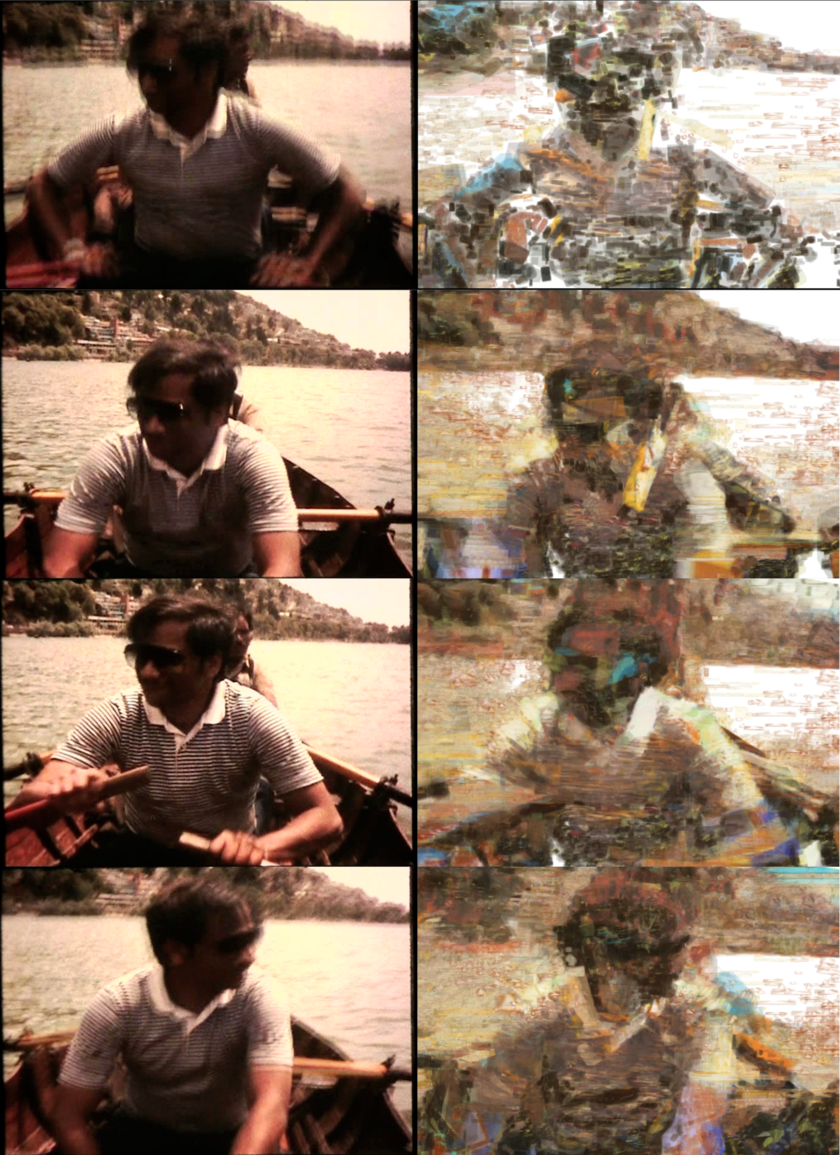
\includegraphics[width=2.8in]{images/dad-rowing-4x2.png}
  \caption{Left: 4 frames from a target video; Right: Stylization using Paul Klee's corpus in Figure-\ref{fig:cows-klee}.  We aim to synthesize with greater expression and less abstraction, and allow the minimum region size to be very small. Best viewed in the color manuscript at 200\% or in the video online. Photos by the author.}
  \label{fig:rowing}
\end{figure}
Two examples in video-based stylization are presented: one of a subject rowing a boat and another of abstract imagery.  In Figure-\ref{fig:rowing}, we can see 4 frames taken from a video stylization.  We use the same corpus as in Figure-\ref{fig:cows-klee} and allow the minimum region size to be very small, resulting in a more Expressionist style.  The first frame is not as composed as the later frames, as there will have only been 1 frame of compositing.  As a result, the first frame in video-based Expressionist stylization may not be a consistent style with its later frames.
\subsection{Video: Abstract}\vspace{-0.4em}
\begin{figure}[ht]
  \centering
  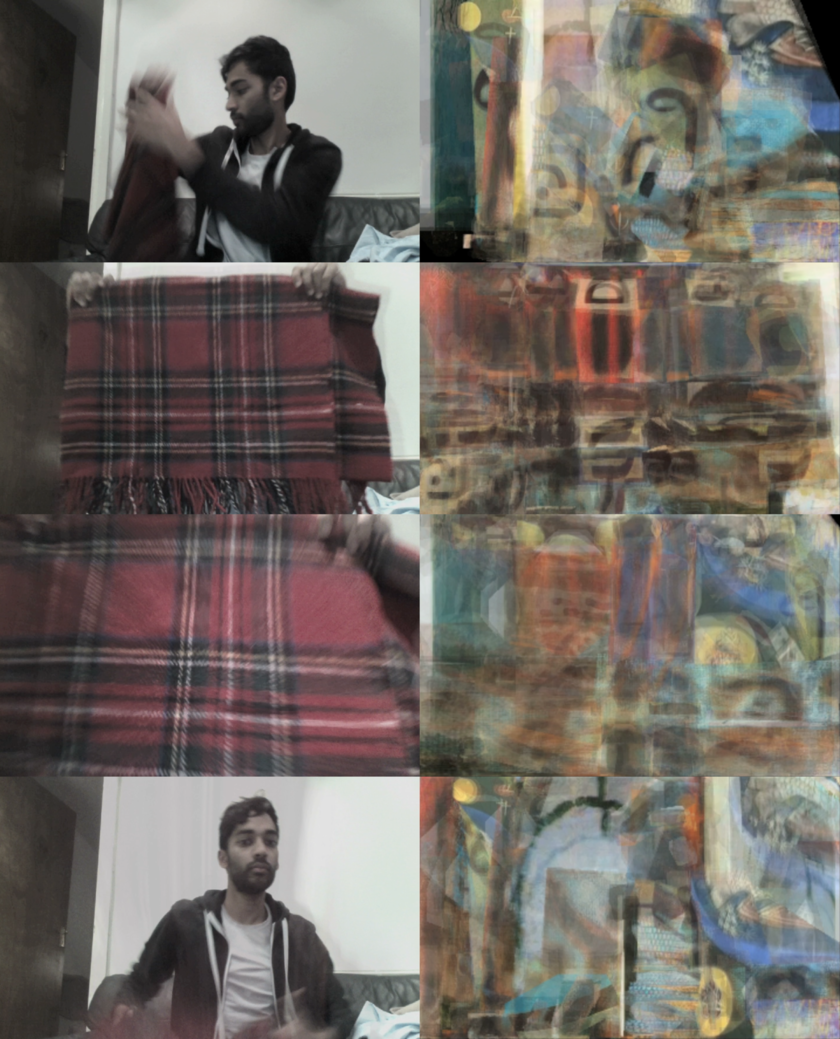
\includegraphics[width=2.8in]{images/blanket-video.png}
  \caption{Left: 4 frames from a target video; Right: Stylization using Paul Klee's corpus in Figure-\ref{fig:cows-klee}.  Here we aim to stylize with greater abstraction than in Figure-\ref{fig:rowing}, and set the minimum region size to be fairly large. Best viewed in the color manuscript at 200\% or in the video online.   Photos by the author.}
  \label{fig:blanket-video}
\end{figure}
In Figure-\ref{fig:blanket-video}, we stylize a video using the same corpus as in Figure-\ref{fig:cows-klee} and set the minimum region size to be very large.  Thus, instead of producing an Expressionist style as in Figure-\ref{fig:rowing}, less details are synthesized resulting in a more abstract style.  The first frame in this video does not necessarily require more than 1 iteration as it is synthesizing very large regions that often also overlap.
\subsection{Memory Mosaicing}\vspace{-0.4em}
% picture of memory mosaicing as video thumbnails

The artistic stylization process can be used in a real-time context without an explicit corpus.  In this case, we aggregate representations learned from the ongoing stream of target frames.  Parameters are generally set by the user interacting with the process, or contained to a single preset.  In particular, restricting the total number of representations as first-in-first-out queue allows the process to continue in real-time with a simple linear search index.  In the examples shown in Figure \ref{fig:memory-mosaicing}, we show two example outputs from the same camera stream.  In the left image, we aim for large region sizes and low timesteps, resulting in a more abstract style, reminiscent of Cubist style paintings.  In the right example, we allow higher timesteps and only small region sizes, resulting in a more expressive style similar to paintings in Abstract Expressionism.  
\subsection{Augmented Reality Hallucination}\vspace{-0.4em}
% picture of exhibition setup, still of hallucination with kid in foreground
An interesting case of ``Memory Mosaicing'' is when a participant can actively explore a visual scene.  By using augmented reality goggles, we allowed participants to explore their environment through the our proposed stylization process during an exhibition called ``Augmented Reality Hallucinations'' held at the Victoria and Albert Museum in London.  Participants were invited to wear the goggles where two small CRT screens presented the same output of a ``Memory Mosaicing'' of a single camera mounted on the goggles right eye that faced the scene in front of them (see Figure \ref{fig:vam}).  As the only user interaction was in exploring a scene, a single preset was defined based on large region sizes and low number of timesteps, as shown in the left column in Figure \ref{fig:memory-mosaicing}.  

Participants were also invited to give quantitative and qualitative feedback on their experience.  The summary of the quantitative feedback is shown in Figure \ref{fig:vam-graphics-bar}.  On the feedback form, when participants were asked, ``Did this experience make you think of anything you had seen or heard before?'', three participants made references to their experiences on hallucinogens and two to dreams.  Also of note in the qualitative feedback was references to art styles such as, ``It reminded me of Francis Bacon's Figurative style'' and ``The movement was Impressionistic, almost painterly''.  When asked, ``What did you dislike most about the experience?'', of note were the responses, ``Would have liked more depth in colour'', ``Not sure what I was seeing at first with the goggles'', and ``Hard to understand how it works.''  The lack of understanding of the process may also be revealed in the quantitative analysis in the second bar of the graph.  However, on average, this number is still quite high across participants, though there is also no baseline to compare to.  
\section{Discussion and Future Works}
We have presented a framework for producing artistic stylizations of images or videos.  A corpus of image material is automatically segmented, defining the possible strokes effecting the possible colors and textures in the stylization.  Using a simple set of parameters, we have shown that many stylizations of a target image or video are possible, ranging from Impressionism, Expressionism, and Abstract Expressionism.  By allowing the interactive refinement of an image's stylization, we allow the user to experiment with a range of stylizations through simple parameters.  This interactive refinement affords compositing, the ability to blend together stylizations from different parameters over time.  We also demonstrate the extension of this framework to video-based stylization using simple motion tracking.  As in image-based stylization, the user can influence the stylization through the same set of parameters in real-time to interactively refine the stylization.  

The extension of video-based stylization is also particularly suited for real-time contexts as shown in ``Memory Mosaicing'', where a database is aggregated from learning representations in a target frame over time.  Extending this case to an augmented reality setting, a participant of this system can actively view their world, creating a hallucinogenic experience, as validated by a number of participants during an exhibition at the Victoria and Albert Museum.  However, the feedback from this installation also revealed a lack of understanding in how the process works.  

A number of issues could be addressed in future versions.  For instance, synthesized regions with poor shape matches can be heavily distorted in a resulting synthesis.  In these cases, it is likely that the database did not include any other matches with more similar shapes, or the shape descriptor had been weighted too low.  As well, the speed of the synthesis in a real-time context can be greatly improved with other search methods such as tree or hash-table based indexes.  As well, our approach to addressing the temporal coherence of the resulting stylization may be improved with investigating incorporating more recent models of optical flow, keyframe detection, and possibly spatiotemporal detection of representations rather than purely spatial ones.   
%\section*{Acknowledgements}
%Thanks to Baptiste Caramiaux and Atau Tanaka for their comments on an earlier draft.  Also thanks to Enrica Cassentini for her help in creating a children's painting and earlier tests in stylization.  
%%% Please use the ``acmsiggraph'' BibTeX style to properly format your
%%% bibliography.

\begin{figure}[h]
  \centering
  \includegraphics[width=2.8in]{images/memory-mosaic-2x2.png}
  \caption{2 examples of ``Memory Mosaicing'' showing the input (top) and resulting real-time stylization (bottom).   Photos by the author.}
  \label{fig:memory-mosaicing}
\end{figure}
\begin{figure}[h]
  \centering
  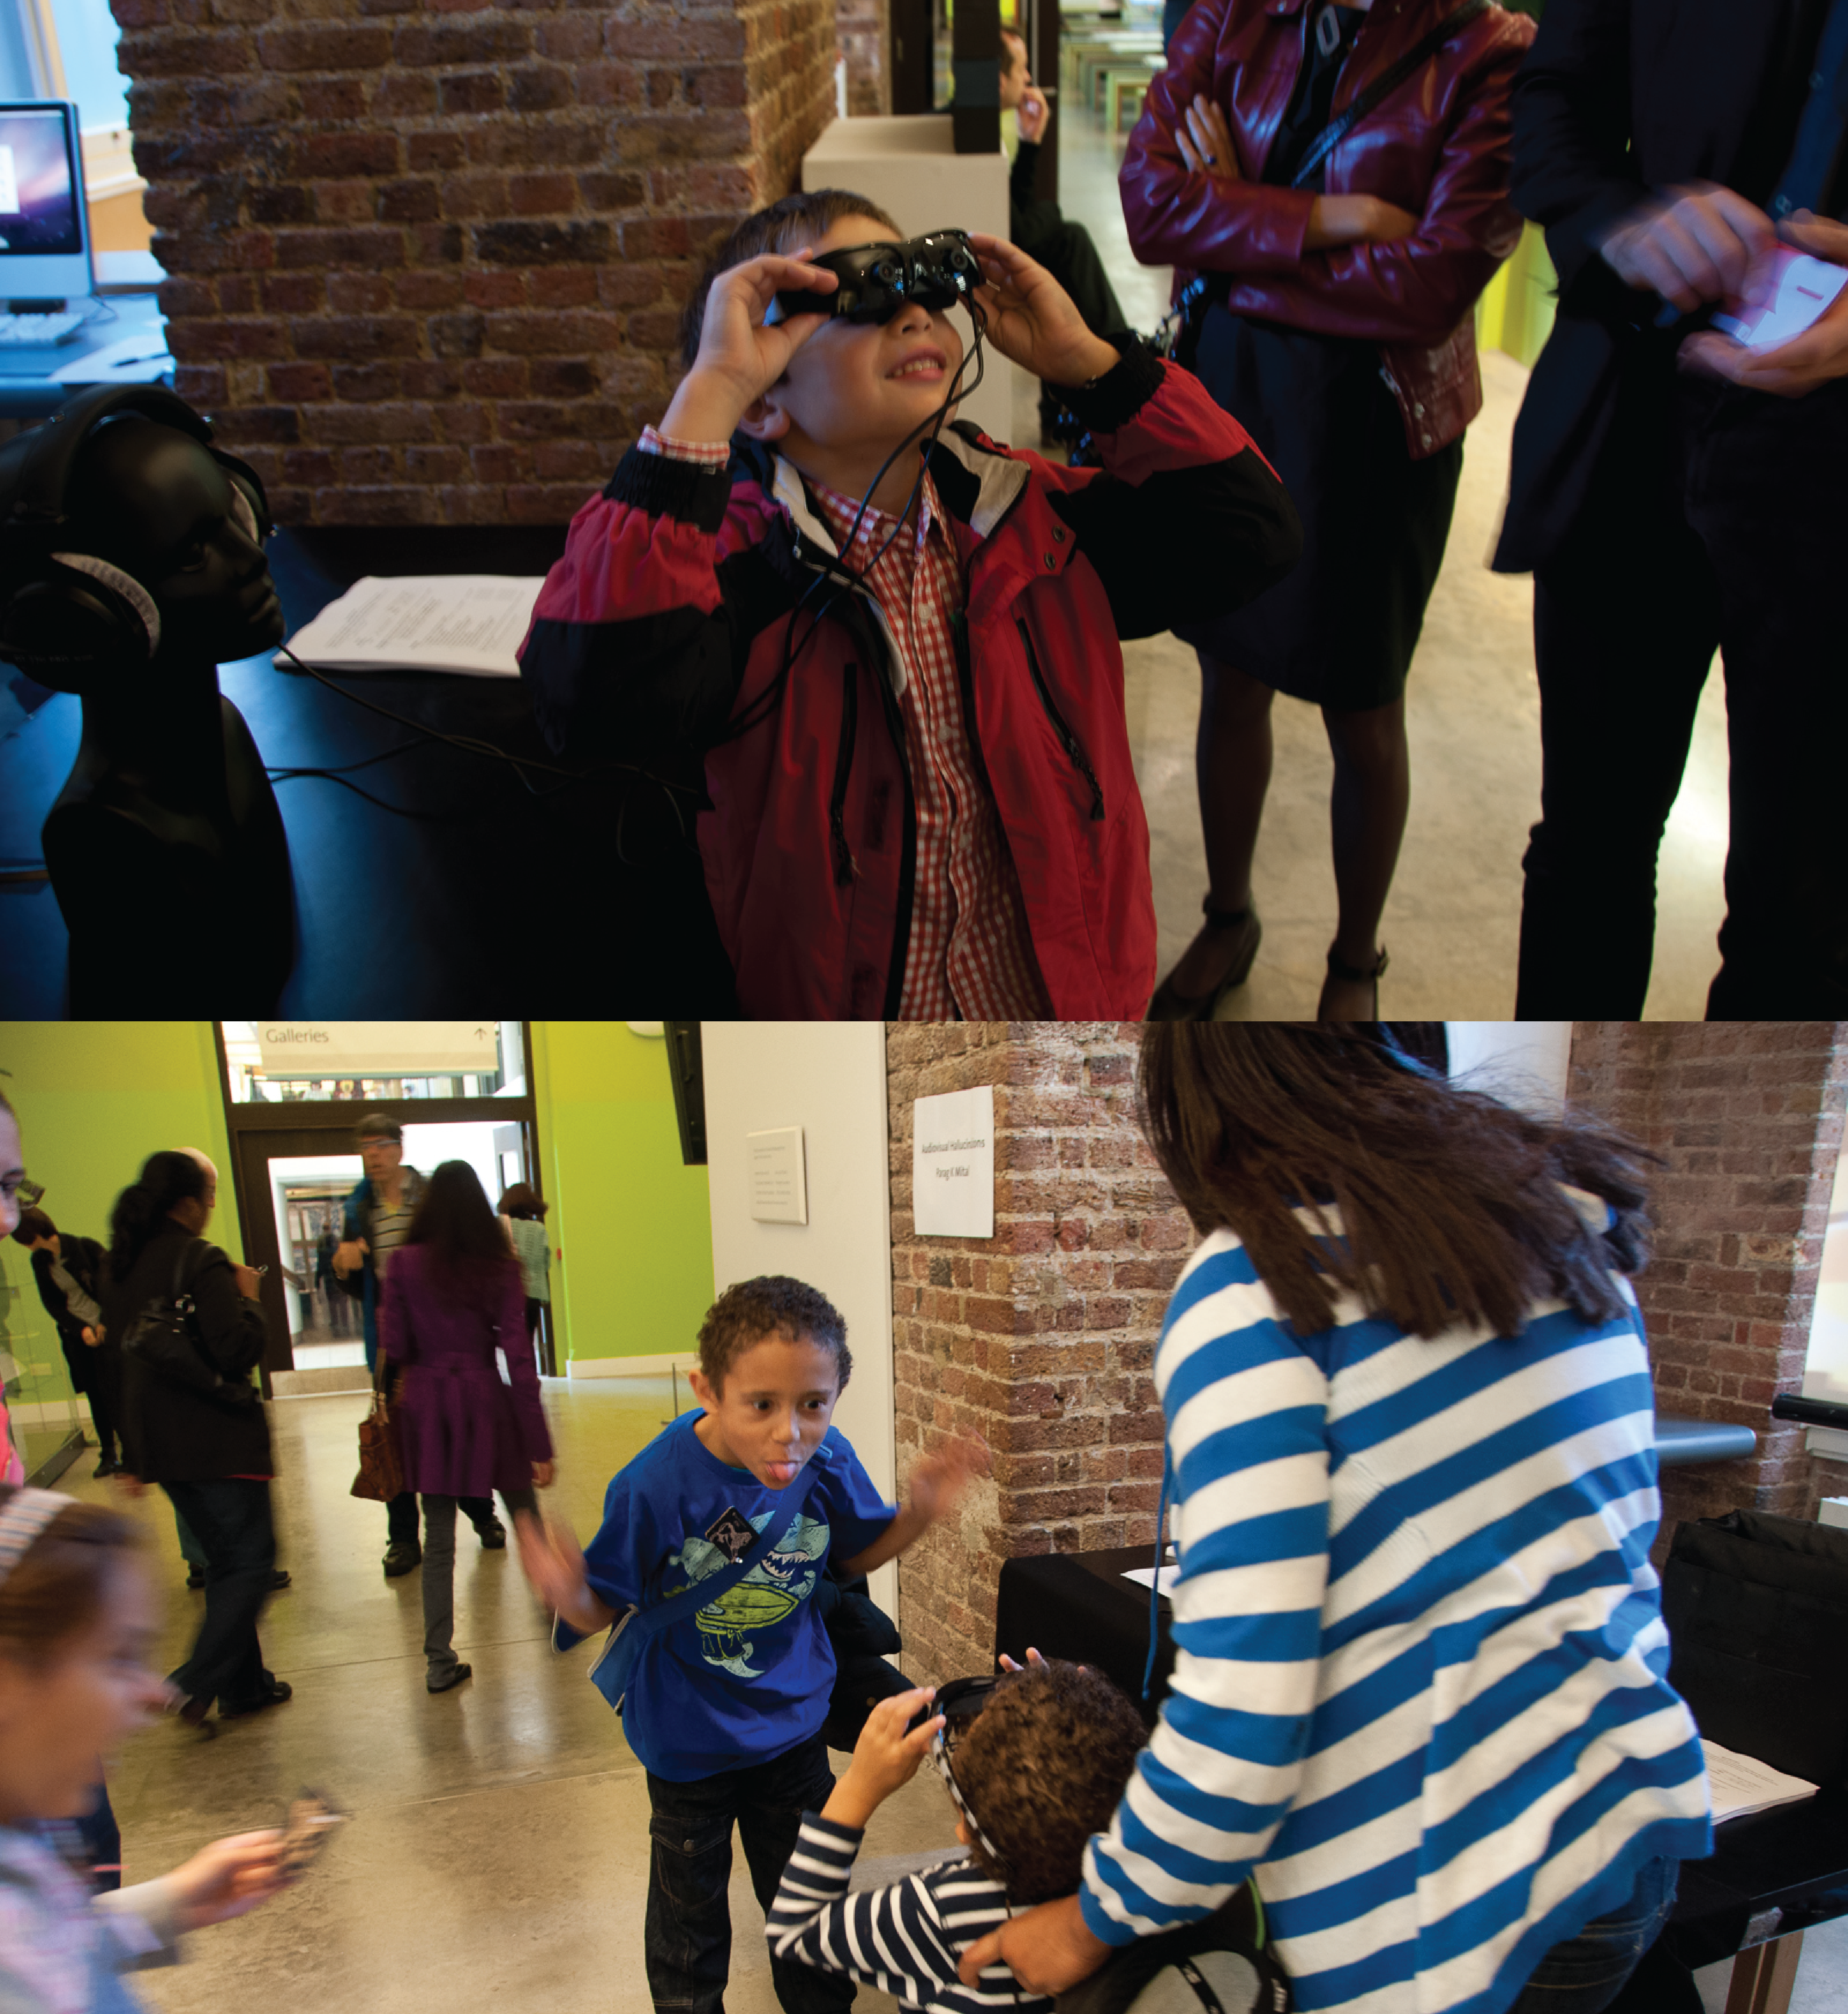
\includegraphics[width=2.4in]{images/vam.png}
  \caption{An exhibition at the Victoria and Albert Museum in London had participants wear Augmented Reality goggles with software running a real-time version of ``Memory Mosaicing''.  Photos by the author.}
  \label{fig:vam}
\end{figure}
\begin{figure}[h]
  \centering
  \includegraphics[width=2.4in]{images/vam-graphics-bar-resize-01.png}
  \caption{Results of the ``Augmented Reality Hallucination'' installation feedback where 21 participants were asked to rate different aspects of the visual synthesis.  Error bars depict +/- 1 S.E.}
  \label{fig:vam-graphics-bar}
\end{figure}

